% Final research paper, IEEE conference format, author-year citations.
% Build:  make        (pdflatex, bibtex, pdflatex, pdflatex)
% Figures: .venv/bin/python tools/paper_figures.py  (from the repository root)
\documentclass[conference,a4paper]{IEEEtran}

\usepackage[T1]{fontenc}
\usepackage{amsmath,amssymb}
\usepackage{graphicx}
\usepackage{pdfpages}
\usepackage{booktabs}
\usepackage{multirow}
\usepackage{xcolor}
\usepackage{url}
\usepackage{tikz}
\usetikzlibrary{arrows.meta,positioning,fit}
\usepackage[hidelinks]{hyperref}

% Author-year citations (Wits named style, as in the proposal).
\usepackage{natbib}
% Force natbib.sty to put citation labels in the reference list
\makeatletter
\renewcommand\NAT@biblabel[1]{\def\citeauthoryear##1##2{##1 ##2}[#1]\hfill}
\renewcommand\NAT@bibsetup[1]{%
  \setlength{\itemsep}{\bibsep}\setlength{\parsep}{\z@}}
\def\@lbibitem[#1]#2{%
  \if\relax\@extra@b@citeb\relax\else
    \@ifundefined{br@#2\@extra@b@citeb}{}{%
     \@namedef{br@#2}{\@nameuse{br@#2\@extra@b@citeb}}}\fi
   \@ifundefined{b@#2\@extra@b@citeb}{\def\NAT@num{}}{\NAT@parse{#2}}%
   \item[\hfil\hyper@natanchorstart{#2\@extra@b@citeb}\@biblabel{#1}%
    \hyper@natanchorend]%
    \NAT@ifcmd#1(@)(@)\@nil{#2}}
\makeatother


\bibliographystyle{named-wits}
\bibpunct{[}{]}{;}{a}{}{}
\renewcommand{\bibfont}{\footnotesize}
\setlength{\bibsep}{1.5pt}

\graphicspath{{figures/}}
\newcommand{\code}[1]{\texttt{\small #1}}

\begin{document}

\title{How Far Can a Digital Twin of a Low-Cost Robot Be Trusted?\\
A Preregistered Comparison of a Coupled Electrical and\\ Dynamic Twin with Two Real Robots}

\author{\IEEEauthorblockN{Muthuphei Mukhunyeledzi, Branden Ingram and Pravesh Ranchod}
\IEEEauthorblockA{School of Computer Science and Applied Mathematics\\
University of the Witwatersrand, Johannesburg, South Africa}}

\maketitle

\begin{abstract}
A robot moves only as well as its circuit lets it, yet robot simulators
command a motor's torque or speed without modelling the supply that drives
it. We build a digital twin of the
Waveshare JetBot in which a circuit-level model of the power electronics,
written in \emph{elecsim}, a code-first simulation framework we develop, is
solved together with the robot's dynamics at every step. We verify elecsim
against ngspice and test the twin against two physical robots with
predictions saved in advance and a preregistered fifty-run test. Our research
shows that the coupled twin predicts steady motion to within a few percent,
including held-out spins on a second robot to within 0.5\%. An ablation shows
what the coupling contributes: a twin with an ideal supply, calibrated the
same way, misses the same spins by 4.9\% because it cannot follow the
battery's charge, and cannot predict the Jetson's supply falling to 4.53\,V,
below its specification, which the coupled twin predicts to 4\,mV. Over fifty
straights the twin passes the preregistered test yet is 8\% short on every
run that goes straight; separating the caster's rolling and scrubbing
friction reduces this to 0.9\%, and cross-validation over all batches keeps
it within 1.3\%. Short open-loop turns are not predicted on either robot, and
the robots' occasional swerves are traced to a sustained wheel-speed
difference, not a timing fault.
\end{abstract}

\begin{IEEEkeywords}
digital twin, reality gap, electromechanical co-simulation, model validation,
differential-drive robot, preregistration
\end{IEEEkeywords}

% =====================================================================
\section{Introduction}

A \emph{digital twin} is a virtual model of a specific physical system that
is kept close enough to it to stand in for it: to predict its behaviour, to
test changes before they are made, or to detect when the real system departs
from what is expected \citep{grieves2017digital,tao2019digital}. Reviews of
the field find that few published twins exchange data with their physical
system in both directions \citep{kritzinger2018digital}, and that the
benefits claimed for twins are rarely validated or quantified
\citep{jones2020characterising}. In robotics the mismatch between simulated
and real behaviour is the \emph{reality gap}
\citep{jakobi1995noise,koos2013transferability}. It is usually worked around
by randomising the simulator \citep{tobin2017domain,peng2018sim}, and there
is no common benchmark for measuring it \citep{muratore2022robot}.

A physical robot is an electrical system as much as a mechanical one. Its
motors turn only as fast as the battery, the protection circuit, the switch
and the driver chip allow; when the battery runs down or the processor draws
more power, the motion changes. Robot simulators nevertheless drive a motor
by a force, torque or velocity command \citep{koenig2004design,todorov2012mujoco},
without its voltage, current and back-EMF, and circuit simulators stop at the motor terminals \citep{nagel1973spice}. We
build a twin in which the two are one system: at every step the circuit is
solved for the motor currents given the wheel speeds, and the dynamics move
the robot given those currents. The circuit model shows whether the
electronics are working, and the coupling shows what their state does to the
robot's motion.

We study the question on a small, inexpensive robot: \emph{how far can a
digital twin of a low-cost mobile robot be trusted, where does it fail, and
what does modelling the circuit add?} The platform is the Waveshare JetBot
AI Kit \citep{waveshare2020jetbot}, a two-wheel educational robot built
around an NVIDIA Jetson Nano \citep{nvidia2019jetbot}. The project began as
the design of a RoboCup Small Size League robot \citep{kitano1997robocup};
when parts could not be obtained in time, it was redirected to a robot that
exists, so that the twin can be judged by whether it is right rather than by
whether it looks plausible. Our contributions are:
\begin{enumerate}
\item \emph{elecsim}, a Python framework in which a circuit, its ratings and
  its requirements are code, verified against ngspice (Section~\ref{sec:system}).
\item A JetBot twin that couples the board's power path to the robot's
  dynamics and exposes the robot's own software interface.
\item A validation protocol that keeps the comparison a test rather than a
  fit: provenance, saved predictions, staged calibration, held-out and
  preregistered tests, and cross-validation (Section~\ref{sec:method}).
\item Results on two robots that locate where the twin can be trusted, an
  ablation that isolates what the electrical coupling contributes, and two
  model diagnoses, of the caster and of the swerves (Section~\ref{sec:results}).
\end{enumerate}

% =====================================================================
\section{Related Work}\label{sec:related}

\subsection{Digital twins}
\citet{grieves2017digital} define a digital twin as a virtual representation
linked to a physical product throughout its life. \citet{kritzinger2018digital}
distinguish a \emph{digital model}, a \emph{digital shadow} (data flow from
the physical object only) and a full twin (data flow both ways), and find
that most manufacturing ``twins'' are models or shadows. Later reviews
name levels of fidelity \citep{jones2020characterising} and model validation
\citep{fuller2020digital} as open problems, and \citet{rasheed2020digital}
argue that physics-based models generalise to problems governed by the same
physics but can carry large errors from uncertain inputs, so they should be
combined with measured data. In these terms our twin is a
digital shadow: the robot's logs condition every replay, but the twin does
not command the robot. We focus on measured agreement between the twin and
its robot.

\subsection{The reality gap}
\citet{jakobi1995noise} popularise the term and show that realistic noise in
a simulation helps evolved controllers transfer to the real robot;
\citet{koos2013transferability} learn which simulated behaviours transfer.
Sim-to-real work in learning-based control randomises the simulator's
appearance \citep{tobin2017domain} or dynamics
\citep{peng2018sim,muratore2022robot} so that what is learned is robust to the
gap, or improves the actuator model, analytically with a DC-motor model
\citep{tan2018sim} or with a network learned from data
\citep{hwangbo2019learning}. Surveys \citep{zhao2020sim,muratore2022robot}
catalogue the methods for crossing the gap, chiefly domain randomisation;
\citet{muratore2022robot} note that there is no common benchmark for
sim-to-real transfer and that physics-engine comparisons cover few scenarios,
and \citet{choi2021use} identify validated simulation, and models of contact
and friction, as central open challenges. We do not train a controller; we measure the gap of
one deterministic model term by term.

\subsection{Simulators and circuit models}
Gazebo \citep{koenig2004design} and MuJoCo \citep{todorov2012mujoco} model
rigid-body dynamics and contact; no engine is best on every test
\citep{erez2015simulation}, and contact remains hard to simulate accurately
\citep{erez2015simulation,collins2021review}. None models the electrical supply. Circuit simulators
descend from SPICE \citep{nagel1973spice} and solve modified nodal analysis
(MNA) \citep{ho1975modified}. Acausal languages such as Modelica
\citep{fritzson2014principles} can couple electrical and mechanical domains
but need a dedicated toolchain. elecsim uses MNA, but parts, ratings and
requirements are ordinary Python, so a design is tested and versioned like
any other code and can be stepped inside a robot simulation loop.

\subsection{Calibration and validation}
System identification \citep{ljung1999system} estimates model parameters from
experiments. \citet{kennedy2001bayesian} show that even the best-fitting
parameters of an inadequate model leave a systematic discrepancy, and
\citet{brynjarsdottir2014learning} show that calibrating without accounting
for it biases the parameters: a wrong model compensates by moving the wrong
numbers. The verification and validation literature
\citep{oberkampf2010verification,sargent2013verification} separates
calibration from validation data. For wheeled robots,
\citet{borenstein1996measurement} separate systematic from non-systematic
odometry errors by repeated runs, and \citet{siegwart2011introduction} list
wheel slip and uneven floor contact among the non-systematic error sources. Preregistering hypotheses
and analyses \citep{nosek2018preregistration} guards against the data-dependent
choices that make an analysis agree with its data
\citep{gelman2014statistical}. We adopt it for the main test.

% =====================================================================
\section{System}\label{sec:system}

\subsection{elecsim: a code-first electrical framework}
A design in elecsim is a Python module whose \code{build()} function returns a
circuit. A \emph{component} is a class that declares its ports and parameters
and supplies \code{stamp}, which adds its linearised equations, and
\code{measure}, which names what can be observed about it. A \emph{circuit}
joins components into nets. \emph{Constraints} are of three kinds:
\emph{rules} check the wiring without simulating, \emph{limits} compare each
signal with a component's rating at every step, and \emph{requirements} ask
whether a finished run met its purpose (``the 5\,V rail stays above
4.75\,V''). A \emph{report} lists every constraint in every scenario with the
unverified numbers it rests on: every parameter carries its provenance,
\code{datasheet}, \code{measured} or \code{assumed}.

The solver assembles and solves, at each Newton iteration,
$\mathbf{G}(\mathbf{x}_k)\,\Delta\mathbf{x} = -\mathbf{f}(\mathbf{x}_k)$
\citep{ho1975modified}, with $\mathbf{x}$ the node voltages and any branch
currents, and steps in time by backward Euler with automatic step halving. A
damped retry and a fallback in which regulators that lose their input switch
off make it robust to parts written by non-specialists. The library covers
passives, sources, diodes, MOSFET switches, a lithium cell with a
state-of-charge curve, a pack protector, a buck converter, a DC motor, an
H-bridge, the PCA9685 PWM controller and measurement chips with their real
resolution. An averaged H-bridge solves the periodic winding current in closed
form, correct in discontinuous conduction and in both decay modes, and within
3\% of the switching model; with it the twin runs at about three times real
time. Sixty automated tests cover the framework.

\subsection{The coupled JetBot twin}
\begin{figure}[t]
\centering
\begin{tikzpicture}[
  font=\scriptsize, node distance=3mm and 4mm,
  box/.style={draw, rounded corners=2pt, align=center, minimum height=7mm, inner sep=2pt},
  arr/.style={-{Stealth[length=1.6mm]}}]
\node[box] (cmd) {\code{set\_motors}\\(same API)};
\node[box, right=of cmd] (pwm) {PCA9685\\registers};
\node[box, right=of pwm] (circ) {power path\\(elecsim, MNA)};
\node[box, right=of circ] (dyn) {dynamics\\motors, tyres,\\caster, body};
\node[box, below=5mm of circ] (sens) {sensor models\\INA219, Jetson monitor};
\node[box, below=5mm of dyn] (pose) {pose, wheel\\speeds};
\draw[arr] (cmd) -- (pwm);
\draw[arr] (pwm) -- (circ);
\draw[arr] ([yshift=1.5mm]circ.east) -- node[above, font=\tiny]{$i$} ([yshift=1.5mm]dyn.west);
\draw[arr] ([yshift=-1.5mm]dyn.west) -- node[below, font=\tiny]{$\omega$} ([yshift=-1.5mm]circ.east);
\draw[arr] (circ) -- (sens);
\draw[arr] (dyn) -- (pose);
\end{tikzpicture}
\caption{The coupled twin. A motor command becomes the same PWM register
writes the real library makes. Each 1\,ms step the circuit is solved for the
motor currents $i$ given the wheel speeds $\omega$ (back-EMF), and the
dynamics advance the robot under the resulting torques.}
\label{fig:arch}
\end{figure}

The expansion board's schematic is transcribed component by component: three
18650 cells and their holder, the protection circuit, the current-sense shunt
and INA219 monitor, the slide switch, the buck converter feeding the Jetson,
the PWM controller and the motor drivers. The board has footprints for two
alternative driver chips, a TB6612FNG or two DRV8870s, which treat the motor
differently between PWM pulses; the twin contains both. The Jetson Nano is
written as a new component, the intended way to extend the framework.

The twin's \code{Robot} object has the robot library's methods:
\code{set\_motors(left,~right)} writes the same PCA9685 registers as the real
\code{Motor} class, and a test asserts identical register values. The circuit
and the dynamics are coupled in both directions (Fig.~\ref{fig:arch}): the
wheel speeds set the motors' back-EMF, the circuit returns the winding
currents, and these set the torques. A run-down battery, a heavier Jetson
load or a different driver chip therefore changes the motion through the
same equations as on the robot.

The dynamic state is position, heading, forward speed $v$, yaw rate
$\omega_z$ and the two wheel speeds. Each motor follows the DC model
\citep{hughes2019electric}, reflected through the gearbox with an efficiency,
and each wheel carries the rotor inertia and Coulomb and viscous friction.
Each tyre transmits a force that saturates at its friction limit,
$F = \mu_t N \tanh\!\left((r\omega - v_w)/s_0\right)$, a smooth approximation of the saturating slip curve
\citep{pacejka2012tire}. The caster is a ball at distance $x_c$ behind the
axle whose contact point moves at $(v,\, \omega_z x_c)$ in the body frame. As
first built, it resists with one coefficient $\mu_c$ in every direction;
Section~\ref{sec:refit} shows why this is replaced by
\begin{equation}
f_x = -\mu_\text{roll} N_c \tanh\!\frac{v}{\epsilon},\qquad
f_y = -\mu_\text{scrub} N_c \tanh\!\frac{\omega_z x_c}{\epsilon},
\label{eq:caster}
\end{equation}
with separate resistance to rolling along the heading and to scrubbing
across it; with $\mu_\text{roll}$ unset the model reduces to the original.
Load transfer between wheels and caster is included; sideways tyre slip,
gearbox backlash and differences between the motors are not. Geometry comes
from the manufacturer's CAD model, which also drives a browser viewer
(Fig.~\ref{fig:viewer}) that shows the robot moving beside the power path's
live currents and voltages and every part against its rating, so the effect
of the circuit on the motion can be watched as it happens.

\begin{figure}[t]
\centering
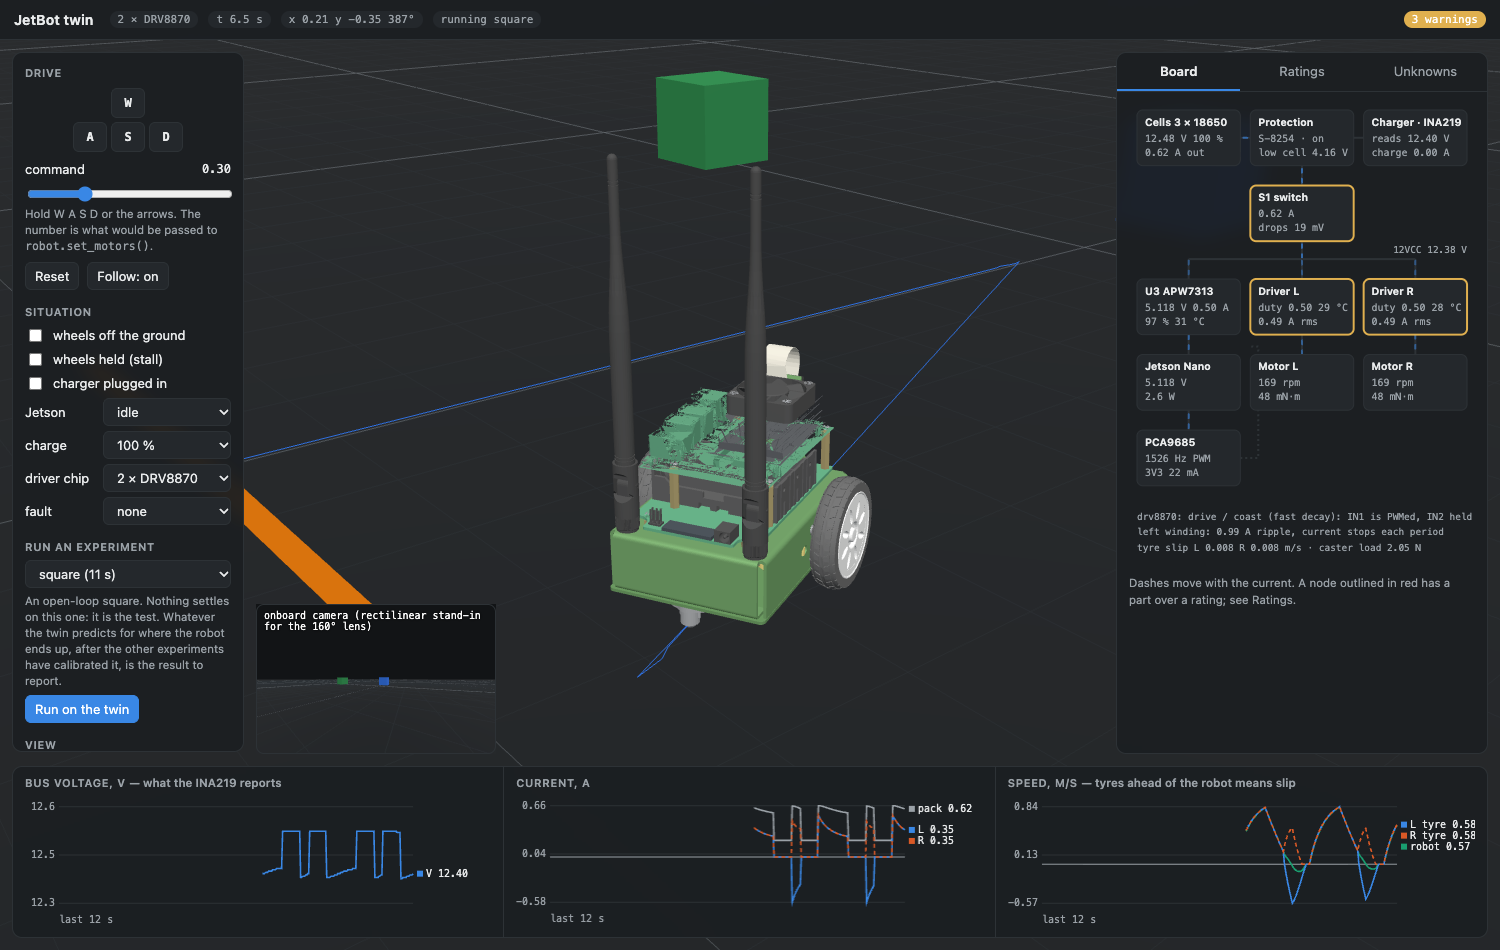
\includegraphics[width=\columnwidth]{viewer.png}
\caption{The live twin in the browser: the manufacturer's CAD, the board's
power path with live currents and voltages, and traces of what the robot's
own sensors would report. All values come from the coupled Python twin.}
\label{fig:viewer}
\end{figure}

% =====================================================================
\section{Methodology}\label{sec:method}

\subsection{Research questions}
\begin{description}
\item[RQ1] How closely does the twin, built from documentation and calibrated
  in isolated stages, predict the robot before each run?
\item[RQ2] Does the twin fall within the robot's own variation over many
  repeats of one manoeuvre?
\item[RQ3] Where the twin fails, can the cause be located in the model?
\item[RQ4] What does coupling the circuit to the dynamics add?
\end{description}

\subsection{What can be observed}
A twin can only be compared with a robot through the robot's sensors. The
JetBot measures its battery rail voltage (INA219) and the Jetson reports its
own input voltage and power. The INA219's shunt lies between the charger jack
and the battery rail, so the robot cannot measure its own load or motor
current, wheel speed or position. The twin reports what each real sensor
would report, at its resolution; everything else is measured from video:
wheel speed from a marker on the hub, paths using the 50\,cm floor tiles as a
ruler, and turn angles from the robot's boards at rest.

\subsection{Protocol}
\emph{Provenance.} Every number is tagged as datasheet, measured or assumed,
and the assumed ones are printed with every result.
\emph{Predictions before measurement.} Before the robot is powered, forty
twins drawn from the uncertainty of the assumed parameters give a 5--95\%
band for every experiment; before each floor run, the calibrated twin's
prediction is saved.
\emph{Staged calibration.} Each experiment isolates a few parameters
(Table~\ref{tab:experiments}), fitted by least squares with the rest held.
Geometry is measured and never fitted, and the driver chip is identified by a
direct electrical test, because a rehearsal shows that a free fit chooses both
wrongly.
\emph{Held-out tests.} An open-loop square fits nothing; on the second robot,
the fifty straights fit nothing in the first round. Each real run is compared
with the twin \emph{replayed} on that run's conditions: the command times as
executed, the Jetson power logged, and the state of charge implied by the
resting voltage.

\begin{table}[t]
\caption{Experiments and the parameters each isolates}
\label{tab:experiments}
\centering\footnotesize
\begin{tabular}{@{}lll@{}}
\toprule
Experiment & Set-up & Settles \\
\midrule
CPU load step & bench & pack and 5\,V path resistance \\
driver test & wheels up & which driver chip is fitted \\
wheels-up sweep & wheels up & motor constant, friction \\
stall & wheels held & winding resistance \\
spin & floor & caster friction \\
straight & floor & drag on the floor \\
square, short turns & floor & nothing (held out) \\
50 straights (robot 2) & floor & nothing (preregistered) \\
\bottomrule
\end{tabular}
\end{table}

\emph{Rehearsal.} Before touching hardware, the procedure is run against a
second twin with nine parameters moved by 10--45\%, seen through noisy
sensors. It exposes two faults: with the wheel radius free, the fit returns a
10\,mm wheel while still scoring well on the held-out square
\citep{brynjarsdottir2014learning}, and an inferred driver chip is the wrong one.
After both fixes the procedure recovers every altered value to within 9\%.

\subsection{The preregistered test on robot 2}
After robot 1 develops a fault, a second unit is calibrated from its own bench
and spin experiments. Before its first straight run we commit the prediction
and the test: both wheels at 0.5 for 1.5\,s from rest, fifty times in ten
batches of five, filmed from 1.01\,m. The planned analyses are (1) a spread
test, passed if zero lies within the middle 95\% of the residuals
$d_i = \text{robot}_i - \text{twin}_i$; (2) the bias, with a 95\%
$t$-interval over batch means; (3) spread within and between batches; and
(4) drift and heading, reported only. No run is excluded. Positions come from
a video tool that uses the tile joints as a ruler (2.4\,mm RMS) and corrects
for the robot's height using its LED, 8.5\,cm above the floor, leaving about
$\pm0.5\%$ uncertainty.

\subsection{Coupling ablation and cross-validation}
To answer RQ4 we build three twins that differ only in what the motors are
fed: the \emph{coupled} twin; a \emph{no-sag} twin, whose power path has no
resistance but still follows the battery's charge; and an \emph{ideal-supply}
twin, also fixed at full charge, as a robot simulator without an electrical
model would assume. Each goes through the same calibration (motor constant
from the wheels-up sweep, caster scrubbing from two spins, rolling from
straights 1--5) and the same held-out tests, so none starts at a disadvantage.
To test whether the caster fit depends on which runs it uses, we repeat it
with each batch of five as the fit set and the other 45 runs as the test.

% =====================================================================
\section{Results}\label{sec:results}

\subsection{Verifying elecsim against SPICE}
Table~\ref{tab:spice} compares elecsim with ngspice on five circuits, the
last a copy of the JetBot's power path with robot 2's measured values as both
stalled motors are switched on. DC solutions agree to solver precision. In
transients the error falls in proportion to the step, as backward Euler
should (slope 0.98 on the RC circuit), and the method's known numerical
damping shows on the lightly damped RLC circuit. At the twin's 1\,ms step,
elecsim misses the winding's first millisecond of current rise, whose time
constant is 0.6\,ms; within 5\,ms it agrees with SPICE to 4\,mV on a 2.5\,V
swing. Reducing the twin's step eightfold changes its predicted straight by
0.2\,mm and its spin by 0.2$^\circ$, so the motion predictions do not depend
on the step.

\begin{table}[t]
\caption{elecsim against ngspice}
\label{tab:spice}
\centering\footnotesize
\setlength{\tabcolsep}{3pt}
\begin{tabular}{@{}lll@{}}
\toprule
Circuit & Step & Largest difference \\
\midrule
Resistor bridge (DC) & -- & $10^{-8}$\,V \\
Diode and resistor, 0--5\,V & -- & 0.04\% of current \\
RC charge & $\tau/100$ & 0.2\% of swing \\
RLC ring-down & $T/80$ & 3.4\% of swing \\
JetBot power path & 1\,ms & 4\,mV after 5\,ms \\
\bottomrule
\end{tabular}
\end{table}

\subsection{Electrical behaviour (RQ1, RQ3)}
\emph{The driver chip is identified without opening the robot.} Driving the
DRV8870 channels moves nothing; driving the TB6612FNG channels dips the rail
by 204\,mV. The board carries the TB6612FNG, contrary to our initial
assumption, and, as the twin predicts for that chip, the lowest command that
turns a free wheel is 0.10.

\emph{The Jetson's supply sags below its specification.} Under a CPU load
step, which the Jetson's own power monitor makes a known load, the twin built
from the schematic holds the Jetson at 5.12\,V while the Jetson reports
4.50\,V, below its 4.75\,V minimum. Fitting a 0.49\,$\Omega$ resistance between
the regulator and the Jetson, through header pins and carrier traces on no
schematic, reduces the RMS rail error from 80 to 30\,mV. Robot 2 sags to
4.53\,V through 0.52\,$\Omega$, so the sag is a property of the design. The
reading is the Jetson's own and is not yet confirmed with a meter. The pack's
resistance also doubles as it empties (0.058 to 0.125\,$\Omega$ per cell),
which the twin treats as a constant.

\subsection{Motion on robot 1 (RQ1)}
With the wheels in the air, the twin as designed is 14\% from the measured
wheel speed and 8\% after calibration; the predicted bands hold (199--284\,rpm
at a command of 0.5, measured 268). Spin-up and braking times, never fitted,
agree: 80 against 83\,ms and 140 against 162\,ms. Above a command of about
0.8 (0.6 on robot 2) the robot's speed stops rising in proportion, which the
motor model cannot follow, so robot 2's motors are fitted on 0.1--0.6. On the
floor, the twin's saved predictions are 1.47\,m for a 2\,s straight (measured
1.43\,m, 3\%) and 1095$^\circ$ for a 2\,s spin (1033$^\circ$, 6\%).

On the held-out square the twin gets every side to within 3\,cm and misses
the corners by up to 39$^\circ$. Repeating the 0.29\,s corner from rest shows
why in part: a motor command is fourteen I\textsuperscript{2}C writes from
Python, so its duration varies (254 to 362\,ms) and the angle follows it
(correlation 0.82). Fixing the agent's timing reduces the variation from 29
to 2.2\,ms. Twenty-four timed turns then average 94.3$^\circ$ (SD 7.6) against
the twin's 83.7$^\circ$ (Fig.~\ref{fig:turns}a), a 12.6\% bias that no single
parameter explains without breaking the spin or the straight; corners taken
straight after a side vary three times as much (SD 23$^\circ$). A strip of tape
left on one tyre is found late; removing it changes distance and rotation by
under 3\% but reveals a 2.6\% mismatch between the motors that the twin,
with identical motors, cannot produce.

\begin{figure}[t]
\centering
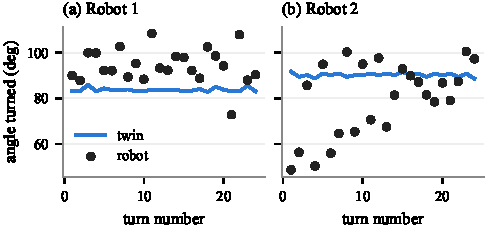
\includegraphics[width=\columnwidth]{turns.pdf}
\caption{Twenty-four identical short turns (0.29\,s at $\mp0.3$, from rest),
robot against the twin replayed on each turn's own timing. Robot 1 turns
12.6\% further than its twin; robot 2 turns 11.6\% less and scatters twice
as much.}
\label{fig:turns}
\end{figure}

\subsection{Fifty straights on robot 2 (RQ2)}
Robot 2 differs measurably from robot 1: 29\% higher cell resistance, 9\%
lower winding resistance, and a caster that drags half again as much (0.506
against 0.324). Table~\ref{tab:straights} gives the preregistered results.
The robot travels 1.120\,m on average and the twin 1.056\,m; zero lies within
the middle 95\% of the residuals ($-6.6$ to $+11.7$\,cm), so \emph{the twin
passes the preregistered spread test}, with a bias of $+6.0\%$ (interval
$+4.6$ to $+8.0$\,cm). Batches do not differ beyond chance.

The data show what the plan does not anticipate (Fig.~\ref{fig:straights}a).
In 10 of the 50 runs the robot swerves hard left on open floor, ending 26 to
49\,cm to the side. We report this split as exploratory. On the 40 runs that
go straight, the robot repeats itself to 1.8\,cm and \emph{the twin is 8.2\%
short on every one}; on these alone the spread test would fail. The test
passes because the swerves widen the robot's spread.

\begin{table}[t]
\caption{Fifty straights on robot 2 (robot minus twin)}
\label{tab:straights}
\centering\footnotesize
\begin{tabular}{@{}lcc@{}}
\toprule
 & Round 1 & Round 2 \\
 & (50 runs) & (runs 6--50) \\
\midrule
Spread test & pass & pass \\
Mean bias & $+6.0\%$ & $-1.5\%$ \\
\quad 95\% interval (cm) & $+4.6$ to $+8.0$ & $-3.5$ to $+0.2$ \\
Runs that go straight & $+8.2\%$ (40) & $+0.9\%$ (35) \\
Runs that swerve (10) & $-2.9\%$ & $-9.6\%$ \\
\bottomrule
\end{tabular}
\end{table}

\begin{figure}[t]
\centering
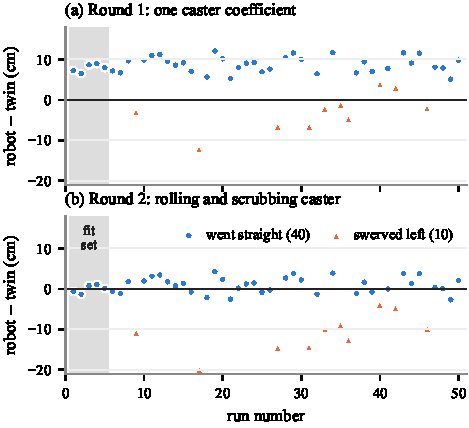
\includegraphics[width=\columnwidth]{straights.pdf}
\caption{Robot minus twin for robot 2's fifty straights. (a) The twin as
calibrated on bench tests and spins. (b) The twin with the caster split into
rolling and scrubbing friction, fitted on runs 1--5 only (shaded). Triangles
mark runs that swerve more than 25\,cm left.}
\label{fig:straights}
\end{figure}

\subsection{Locating and fixing the error (RQ3)}\label{sec:refit}
Robot 2's caster coefficient is fitted on spins, where the ball is dragged
sideways; driving straight, it rolls. Replaying one run with different caster
coefficients gives 1.061\,m at 0.506 (the spin fit), 1.113\,m at 0.324 (robot
1's) and 1.198\,m at 0.02 (a free ball), against 1.144\,m measured, while a
10\% change in gearbox efficiency moves it by only 7\,mm. On robot 1 the
mismatch is hidden because gearbox efficiency and caster friction are fitted
together on a straight and a spin, and the efficiency moves further (0.65 to
0.51) than a gearbox plausibly would to absorb it, as
\citet{brynjarsdottir2014learning} warn.

We therefore separate rolling and scrubbing (Eq.~\ref{eq:caster}), committing
the fit and test before refitting: $\mu_\text{scrub}$ from two spins (0.524),
$\mu_\text{roll}$ from runs 1--5 (0.227). On the 35 held-out runs that go
straight, the error falls from 8.2\% to 0.9\% (Fig.~\ref{fig:straights}b) and
the spread test passes on them alone. Cross-validation shows that this does
not depend on the choice of runs 1--5: fitted on the straight runs of each
batch in turn, $\mu_\text{roll}$ lies between 0.15 and 0.23 and the error on
the other batches' straight runs between $-1.3$ and $+1.0\%$ (nine folds; one
batch has too few straight runs). A 95\% prediction interval from each fit
set's own scatter covers 97\% of held-out straight runs on average, but only
80\% of all runs, because the swerves fall outside it. Fitted on batches that
include swerves, $\mu_\text{roll}$ rises to as much as 0.45. The fitted value
is above a free ball's and absorbs losses the twin does not separate, such as
tyre rolling resistance.

Ten new spins with the corrected twin average 1039$^\circ$ against the twin's
1044$^\circ$ ($-0.5\%$, interval $-16$ to $+6^\circ$). Twenty-four short turns
average 79.8$^\circ$ (SD 16.2) against 90.3$^\circ$, a $-11.6\%$ bias
(Fig.~\ref{fig:turns}b): robot 2 turns less than its twin where robot 1 turns
more, so the short-turn error is not one systematic term.

\subsection{What the electrical coupling adds (RQ4)}
Table~\ref{tab:ablation} gives the ablation. All three twins fit the
wheels-up sweep equally well (1.1\% RMS), and removing the power path's
resistance alone changes no motion prediction: at these currents the sag is
too small to matter for motion. Following the battery's charge does matter.
The sweep is recorded at 11.5\,V, sagging to 10.2\,V under load, and the test
runs at 12.2--12.4\,V. The ideal-supply twin, which cannot tell these apart,
learns a motor 10\% too weak; on the ten held-out spins it is 4.9\% short,
against 0.5\% for the coupled twin, and on the straights it remains 2.3\% short
even with its rolling friction driven to zero, so calibration cannot repair
it. Only the coupled twin predicts the electrical state: the Jetson's supply
under load to 4\,mV, and a bus sag during each straight, although it predicts
81\,mV where the robot shows 149\,mV, which suggests the twin underestimates
the current drawn on the floor.

\begin{table}[t]
\caption{Ablation on robot 2: what the motors are fed (robot minus twin)}
\label{tab:ablation}
\centering\footnotesize
\setlength{\tabcolsep}{3pt}
\begin{tabular}{@{}lccc@{}}
\toprule
 & Coupled & No sag & Ideal supply \\
\midrule
Motor speed at 6\,V (fitted, rpm) & 249 & 248 & 225 \\
Caster rolling (fitted) & 0.230 & 0.252 & 0 (bound) \\
35 held-out straights & $+0.9\%$ & $+0.9\%$ & $+2.3\%$ \\
10 held-out spins & $-0.5\%$ & $-0.6\%$ & $+4.9\%$ \\
24 short turns & $-11.4\%$ & $-11.2\%$ & $-9.5\%$ \\
Bus sag, straights (robot 149\,mV) & 81\,mV & 0 & 0 \\
Jetson 5\,V loaded (robot 4.53\,V) & 4.53\,V & 5.12\,V & 5.12\,V \\
\bottomrule
\end{tabular}
\end{table}

\subsection{Why the robot swerves (RQ3)}
The shape of a swerve shows when the turning happens. If one wheel is slower
for the whole run, the path is an arc and the sideways drift is about half of
distance times turn; if a wheel starts late, the robot turns first and the
drift is about the full product; if a wheel stops early, it turns last and
drifts little. We trace each hypothesis in the twin and match every swerve
to the nearest point on each curve, in units of the video's measurement error
(5\,cm, 5$^\circ$), measuring the twin's path exactly as the video tool
measures the robot's (Fig.~\ref{fig:swerves}). A sustained speed difference
of about 30\% between the wheels matches 9 of the 10 swerves within two
measurement errors (RMS 0.9); a late start matches 2 and an early stop none
(RMS 4.2 and 5.3). The swerves' distance, 1.02\,m, lies between that implied
by a slow left wheel (0.84\,m) and a fast right one (1.19\,m), so the data do
not say which wheel. The cause is therefore something that persists through
the run, such as traction or the caster, not command timing.

\begin{figure}[t]
\centering
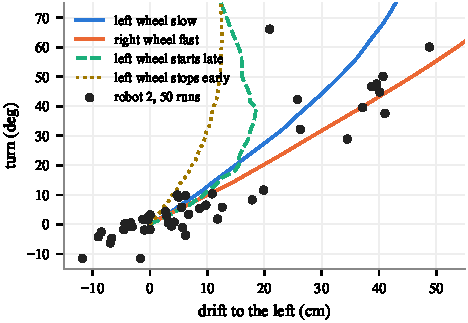
\includegraphics[width=\columnwidth]{swerves.pdf}
\caption{Drift against turn for robot 2's fifty straights, with the path of
each swerve hypothesis traced in the twin. Only a sustained difference
between the wheels passes through the ten swerves. Two turn readings that are
known misreads (92$^\circ$ and 147$^\circ$) lie above the plot.}
\label{fig:swerves}
\end{figure}

\begin{table}[t]
\caption{Twin against robot: summary (robot minus twin)}
\label{tab:summary}
\centering\footnotesize
\setlength{\tabcolsep}{3pt}
\begin{tabular}{@{}p{3.4cm}p{2.4cm}l@{}}
\toprule
Test & Result & Before run? \\
\midrule
Wheel speed, wheels up & 8\% & bands held \\
Spin-up / braking time & 80/83, 140/162\,ms & never fitted \\
R1 straight / 2\,s spin & 3\% / 6\% & yes \\
R1 square: sides / corners & 3\,cm / 39$^\circ$ & yes \\
R1 / R2 short turns & $+12.6\%$ / $-11.6\%$ & yes \\
R2 50 straights, planned test & pass; $+6.0\%$ & preregistered \\
R2 straights, caster fixed & 0.9\% (35 held out) & preregistered fit \\
\quad cross-validated & $-1.3$ to $+1.0\%$ & 9 folds \\
R2 10 spins & $-0.5\%$ & preregistered \\
Jetson 5\,V under load & 4\,mV & fitted \\
Swerves & 30\% wheel difference & diagnosed \\
\bottomrule
\end{tabular}
\end{table}

% =====================================================================
\section{Discussion}\label{sec:discussion}

\emph{Where the twin can be trusted (RQ1).} Our research shows that a
physically based twin of a low-cost robot, built from its documentation and
calibrated in isolated stages, predicts steady behaviour to within a few
percent (Table~\ref{tab:summary}): electrical margins, wheel speed, transient
timing it is never fitted to, spin angle, and straight-line distance once the
caster has the right structure. These are what a designer asks of a twin:
whether a supply is adequate, how fast the robot moves, what a different
driver chip or a flat pack would change.

\emph{Why the circuit belongs in the twin (RQ4).} The ablation shows that the
coupling earns its place for two reasons. The motion depends on the
battery's state, and a twin that cannot follow it is miscalibrated by an
amount no friction coefficient can absorb. And the electrical state is itself
a prediction a robot simulator cannot make: the coupled twin finds the Jetson
running below its rated voltage under load, which no motion test would
reveal. The ablation also shows the limits of the claim: on a charged pack at
moderate commands, the supply's internal resistance does not change the
motion, so the gain comes from the battery's charge, not its sag.

\emph{Where it cannot be trusted.} Short open-loop turns are not predicted on
either robot, and the robots do not repeat them: robot 1 scatters by
$\pm8^\circ$ and robot 2 by $\pm16^\circ$, with biases of opposite sign. A
0.3\,s turn is almost all acceleration and braking, where backlash, the
caster's swivel and bus timing dominate, none of which a lumped model of this
kind captures; the honest output for such manoeuvres is a distribution. The
swerves remain beyond a deterministic twin, but they are now characterised:
a sustained wheel-speed difference of about 30\%, appearing in one run in five.

\emph{A pass is not the whole answer (RQ2).} The preregistered test is passed,
and legitimately, but only because swerves the twin cannot produce widen the
robot's spread; on the runs the twin does describe, it is 8\% short every
time. Reporting the bias and the exploratory split alongside the planned test
is what locates the error. The cause lies in the model's form, one friction
for two kinds of motion, which calibration alone cannot repair
\citep{kennedy2001bayesian} and which randomising a single friction
coefficient \citep{peng2018sim} would not cover; this matches the view
that contact and friction remain among the hardest phenomena to simulate
\citep{erez2015simulation,choi2021use}.

\emph{Threats to validity.} We test two robots on one floor, and robot 2's
fifty runs are made in one 23-minute session. Most bench quantities are
measured once or twice. The swerve split and the form of the caster
correction are chosen after seeing the data, though cross-validation shows the
fitted value is stable. The swerve diagnosis assumes that the video tool's
drift and turn are accurate to 5\,cm and 5$^\circ$. Motor current is never
measured directly, and the twin's under-predicted bus sag suggests the floor
current is underestimated. The robot's mass is estimated from its parts list,
and robot 1's 24 turns are made with tape on one tyre. Several of our own
errors are caught during the work, among them the wheel-radius fit, a logging
fault in the robot's agent, and a height correction that understates every
distance by 4\% until it is checked against the LED; each is caught by a
check built for the purpose.

% =====================================================================
\section{Conclusion}\label{sec:conclusion}

We build a digital twin of the Waveshare JetBot in which a circuit model,
written in the code-first framework elecsim and verified against ngspice, is
solved together with the robot's dynamics, and we test it against two robots
with saved predictions and a preregistered fifty-run test. Our research
shows that the twin can be trusted for steady motion and the electrical
budget, to within a few percent, and cannot be trusted for short open-loop
turns, which the robots themselves do not repeat. Modelling the circuit is
what lets the twin follow the battery's charge, a 4.9\% difference on held-out
spins, and predict the Jetson's under-voltage, which the schematic hides.

The main methodological lesson is that a twin which passes its planned test
can still be consistently wrong, and the error is found only by repeating the
experiment on a second unit and looking past the verdict to the bias. Once
found, it lies in the form of the model, and fixing the form, not retuning a
number, removes it on held-out and cross-validated runs.

Future work should measure motor current directly to resolve the
under-predicted bus sag; model pack resistance as a function of charge;
separate backlash from post-braking state as causes of the turn error;
identify which wheel slows in a swerve with a marker on each hub; and repeat
the fifty straights on other days and on robot 1. The framework, twin, data
and analysis scripts are in the project repository.

\bibliography{references}

% Faculty of Science AI declaration, exported from the .docx in the repo root

\includepdf[pages=-]{ai_declaration.pdf}

\end{document}
